%                                                                 aa.dem
% AA vers. 9.1, LaTeX class for Astronomy & Astrophysics
% demonstration file
%                                                       (c) EDP Sciences
%-----------------------------------------------------------------------
%
%\documentclass[referee]{aa} % for a referee version
%\documentclass[onecolumn]{aa} % for a paper on 1 column  
%\documentclass[longauth]{aa} % for the long lists of affiliations 
%\documentclass[letter]{aa} % for the letters 
%\documentclass[bibyear]{aa} % if the references are not structured 
%                              according to the author-year natbib style

%
\documentclass{aa}  

%
%%%%%%%%%%%%%%%%%%%%%%%%%%%%%%%%%%%%%%%%
\usepackage[normalem]{ulem}
\usepackage{txfonts}
\usepackage{graphicx}
\usepackage{subfigure}
\usepackage{adjustbox}
\usepackage{hyperref}
\usepackage[switch]{lineno}
\hypersetup{
    colorlinks=true,
    linkcolor=blue,
    filecolor=blue,      
    urlcolor=blue,
    citecolor=blue,
    }
%%%%%%%%%%%%%%%%%%%%%%%%%%%%%%%%%%%%%%%%

\newcommand{\fc}[1]{\textcolor{red}{\bf [FC: #1]}}
\newcommand{\af}[1]{\textcolor{green}{\bf [AF: #1]}}
\newcommand{\as}[1]{\textcolor{magenta}{\bf [AS: #1]}}
\newcommand{\al}[1]{\textcolor{cyan}{\bf [AL: #1]}}
%%%%%%%%%%%%%%%%%%%%%%%%%%%%%%%%%%%%%%%%
%\usepackage[options]{hyperref}
% To add links in your PDF file, use the package "hyperref"
% with options according to your LaTeX or PDFLaTeX drivers.
%
\begin{document} 


   \title{Radiation pressure role in accreting massive black hole binaries hydrodynamical simulations}

   %\subtitle{I. Overviewing the $\kappa$-mechanism}

   \author{F. Cocchiararo
          \inst{1,2}\fnmsep\thanks{E-mail: f.cocchiararo@campus.unimib.it} 
          A. Franchini\inst{2,3}\fnmsep\thanks{E-mail: alessia.franchini@uzh.ch}
          A. Lupi \inst{1,2,4}
          A. Sesana \inst{1,2}
          }

   \institute{
    Dipartimento di Fisica "G. Occhialini", Università degli Studi di Milano-Bicocca, Piazza della Scienza 3, 20126 Milano, Italy             
    \and
    INFN, Sezione di Milano-Bicocca, Piazza della Scienza 3, 20126 Milano, Italy
    \and
    Universität Zürich, Institut für Astrophysik, Winterthurerstrasse 190, CH-8057 Zürich, Switzerland
    \and
    DiSAT, Università degli Studi dell’Insubria, via Valleggio 11, I-22100 Como, Italy\\
       }

   \date{}

% \abstract{}{}{}{}{} 
% 5 {} token are mandatory
 
\abstract
% context heading (optional)
% {} leave it empty if necessary  
{}

   \keywords{Accretion, accretion disks --
                Hydrodynamics --
                quasars: supermassive black holes 
               }
   
\titlerunning{}
   \authorrunning{F. Cocchiararo et. al}
   \maketitle
%
%-------------------------------------------------------------------
%%%%%%%%%%%%%%%%% BODY OF PAPER %%%%%%%%%%%%%%%%%%
%%%%%%%%%%%%%%%%% INTRODUCTION %%%%%%%%%%%%%%%%%%
\section{Introduction}
In recent years, the interaction between massive black hole binaries (MBHBs) and their circumbinary disc has been extensively investigated, with the aim of better understanding how the disc affects the binary orbit.%al dynamic and its long-term evolution. 
Despite significant progress, the diversity in numerical methods (e.g. 2D vs 3D codes or grid-based vs Lagrangian codes) and physical models adopted (e.g. locally isothermal vs adiabatic equations of state, inclusion of the disc self-gravity) has resulted in significant discrepancies across the studies. 

A recent study \citep{SantaBarbara2024} investigated a common simple binary-disc setup across multiple simulation codes to measure the magnitude of the gravitational torque that the disc exerts on the binary.% determine the consistency of their results. 
%While general agreement was found on the key aspects of the binary dynamics, some differences arose in the division of the total torque on the binary into contribution from gravitational forces, orbital accretion, and spin accretion.
While the study show general agreement on the sign of the gravitational torque between different codes, there are still significant differences in the magnitude and in other aspects of the binary-disc evolution that essentially depend on the code geometry and on the boundary conditions.

The choice of physical model also affects the results. Gas inflow towards the binary produces shocks at the cavity edge, which modify the  disc's aspect ratio $H/R$ and temperature profile \citep{artymowicz1996, Hayasaki2007, roedig2011, farris2014, Westernacher2023}. Variations in these disc thermodynamic properties directly impact the binary orbital dynamics, with threshold for binary inspiral and outspiral being dependent on the disc aspect ratio \citep{Tiede2020, HeathNixon2020}.
Additionally, self-gravity in circumbinary disc has been shown to regulate both the torque exerted onto the binary and disc's temperature, leading the binary to shrink regardless of its initial temperature - e.i initial aspect ratio - \citep{Cuadra2009, roedig2012, Franchini2021}. 
These simulations and the majority of previous works assumed a locally isothermal equation of state \citep{Franchini2022, Zrake2021,DOrazio2021}, which hold the gas temperature constant over time and limits the ability to capture shock-induced heating and their effect on the disc. 

In contrast, in our earlier work \citep{Cocchiararo2024}, we modelled the circumbinary disc including the self-gravity, employed a live binary model where orbital parameters evolve over time under the influence of gravitational and accretion torques, and included physical cooling in the gas dynamics. These improvements led to more realistic representations of the binary-disc interaction.

A critical aspect often neglected in previous studies is the role of radiation pressure in the hydrodynamic evolution of the circumbinary disc. Radiation pressure plays an important role in the hotter inner regions of the disc, where it significantly affects the gas dynamics and could modifies the disc geometry - including its aspect ratio, cavity shape and eccentricity - and could also alter the inflow of gas towards the binary. This could effect the distribution of torques on the binary, modifying both the accretion rate and the evolution of the binary semi-major axis. 

In this work, we assess the impact of radiation pressure on the hydrodynamic evolution of circumbinary discs around MBHBs. Building on our previous simulations, we implemented the contribution of the radiation pressure in 3D numerical simulations with hyper-Lagrangian refinement approach for milli-parsec scale binaries. The simulations also account for the thermodynamic evolution of the gas using a radiative cooling prescription in the form of black-body radiation. We have also included the disc's self-gravity and the Shakura-Sunyaev prescription for viscosity \citep{ShakuraSunyaev1973}. 
In this live binary model, the thermodynamic evolution of the gas follows an adiabatic equation of state.

We explored the time evolution of binary and disc properties for three systems with eccentricities $e=0, 0.45, 0.9$ and mass ratio $q=1, 0.7, 0.1$, comparing cases with and without radiation pressure.
\fc{in section X there is A, in section Y there is B, etc}





%--------------------------------------------------------------------
%%%%%%%%%%%%%%%%% PHYSICAL SETUP %%%%%%%%%%%%%%%%%%

\section{Numerical and physical model} 

We performed 3D hyper-Lagrangian resolution hydrodynamics simulations of the evolution of the thermal circumbinary disc around accreting MBHB. We used the 3D meshless finite mass (MFM) version of the code \textsc{GIZMO} \citep{Hopkins2015} in combination with the adaptive particle splitting technique \citep[see][for details]{Franchini2022} to have a higher resolution inside the cavity shaped by the binary. We run six different simulations (three of them including the implementation of the radiative pressure) with the following combination of eccentricity $e$ and mass ratio $q$: $e=0$ and $q=1$, $e=0.45$ and $q=0.7$, $e=0.9$ and $q=1$. Each simulation covers 1300 orbital periods. In code unit, the total mass of binary is $M_{\rm B} = M_{\rm 1} + M_{\rm 2} = 1$ where $M_{1}$ and $M_{2}$ are the masses of the primary and secondary black hole respectively, and initial semi-major axis $a_{\rm 0}=1$. Each MBH is modelled as a sink particle with accretion radius $R_{\rm sink} = 0.05a$. As the binary orbit evolves with time \citep{Franchini2023}, mass, linear and angular momentum are conserved during each accretion event, following the method used in the {\sc phantom} code \citep{bate1995}.
Initially, we modelled the circumbinary disc with $N=10^6$ gas particles for a total mass $M_{\rm D} = 0.01 M_{B}$. The mass is distributed with an initial surface density profile $\Sigma \propto R^{-1}$, within a radial range of $R_{\rm in}=2a$ to $R_{\rm out}=10a$. The disc is coplanar with the binary orbit and has an initial aspect ratio $H/R = 0.1$. We generate the initial conditions of the disc using the SPH code {\sc phantom} \citep{Price2017}.

In this work, the thermodynamic evolution of the gas is governed by an adiabatic equation of state with index $\gamma = 5/3$, which allow the disc to heat and cool, capturing the shocks effects. 
We modelled the angular momentum transport within the disc using the $\alpha$ viscosity parameter, which constitutes a simple parameterisation of the turbulence within the disc, as described in the Shakura-Sunyaev accretion disc model. Thus, we included viscosity  through the Shakura-Sunyaev parameterisation with kinematic viscosity $\nu = \alpha c_{\rm s } H$, where $c_{\rm s}$ is the gas sound speed, and set $\alpha=0.1$ in both our simulations. Moreover, because we both included the disc self-gravity and the cooling mechanism, our discs may develop gravitational instabilities (GIs) providing an additional source of angular momentum transport over time \citep{lodatorice2004,Lodatorice2005,lodato2007sg}. To ensure the gravitational stability of the disc, we set the initial Toomre parameter $Q > 1$ \citep{Toomre1964}.


We assume radiative cooling in the form of black-body radiation. The cooling rate is given by: 
\begin{equation}
        \label{eqn:cooling}
        \dot Q = \frac{8}{3} \frac{\sigma_{\rm SB} T_{\rm i}^4}{\kappa \Sigma}
\end{equation}
where $\sigma_{\rm SB}$ is the Stephan-Boltzmann constant, $\kappa$ is the opacity, $\Sigma$ is the disc surface density and $ T_{\rm i} $ is the temperature of each element.
We assume that opacity $\kappa$ is a combination of Kramer opacity $ \kappa_{\rm Kramer} \propto \rho T_{\rm i} ^{-7/2} $ and electron scattering opacity $ \kappa_{\rm es} = 0.2 (1+X) \, \mbox{g}\, \mbox{cm}^2$, with a hydrogen mass fraction $ X=0.59$.
When converted to physical units, all our simulations have a total binary mass $M_{\rm B}= 10^6 M_{\odot}$ and initial separation
$a=4.8 \cdot 10^{-4} \, \rm{pc} \simeq 1.2 \cdot 10^4 \, R_{\rm g}$, where $R_{\rm g} = GM_{\rm B}/c^2$ represents the gravitational radius of the binary. 

\subsection{Radiative pressure in circumbinary disc} 
\label{sec:Prad}

\begin{equation}
    \label{eqn:cons_massa}
    \frac{\partial{\rho}}{\partial{t}} + \nabla(\rho \mathbf{v}) = 0 
\end{equation}
\begin{equation}
    \label{eqn:cons_qm}
    \frac{\partial{(\rho \mathbf{v}})}{\partial{t}} + \nabla[\rho \mathbf{v} \times \mathbf{v}+P] = F_{\rm g} + F_{\rm rad} 
\end{equation}
\begin{equation}
    \label{eqn:var_en}
    \frac{\partial{(\rho \epsilon})}{\partial{t}} + \nabla[(\rho \epsilon + \rho)\mathbf{v}] = - \Lambda + \Gamma - \Lambda_{\rm rad} + \Gamma_{\rm rad}
\end{equation}

\begin{equation}
    \label{eqn:en}
    \epsilon = \rho u + \frac{1}{2}\rho v^2
\end{equation}

\begin{equation}
    \label{eqn:en_withRad}
    \frac{\partial{\epsilon_{\rm rad}}}{\partial{t}} + \nabla \mathbf{F}_{\rm rad} = - \Lambda_{\rm rad} + \Gamma_{\rm rad}
\end{equation}

accoppiamento forte gas e rad (diffusion)
\ref{eqn:var_en}+\ref{eqn:en_withRad}

\begin{equation}
    \epsilon ' = \frac{1}{2}\rho v^2 +\rho u +\rho a T^4
\end{equation}

In {\sc GIZMO}
\begin{equation}
    \epsilon ' = \frac{1}{2}\rho v^2 +\rho (u +a T^4)
\end{equation}

new total energy equation 
\begin{equation}
    \label{eqn:var_en_new}
    \frac{\partial{(\rho \epsilon '})}{\partial{t}} + \nabla[(\rho \epsilon' + \rho)\mathbf{v}] = - \Lambda
\end{equation}

\subsection{Binary angular momentum evolution}
The radiation pressure contribution to the hydrostatic equilibrium of the disc could affect the migration of material from the outer to the inner regions of the circumbinary disc. This could result in a different contribution of the accretion torque $\mathbf{L_{\rm acc}}$ to the total angular momentum equation, potentially changing the binary destiny. Indeed, conservation of angular momentum in our simulations implies that 

\begin{equation}
    \frac{d \mathbf{L}}{dt}=\mathbf{T}_{\rm G} + \frac{d \mathbf{L_{\rm acc}}}{dt}
\end{equation}
where $\mathbf{L}$ is the total binary angular momentum. The contribution from the accretion of gas particles onto the two binary components - $\mathbf{L_{\rm acc}}$ - and the contribution of the gravitational torque exerted by the disc elements onto each individual MBH - $\mathbf{T}_{\rm G}$ -, determine whether the binary shrinks or expands \citep{roedig2012}. 

For each time step, we compute the gravitational torque exerted by N gas particles on each binary component k as 

\begin{equation}
    \mathbf{T}_{\rm G} = \sum_{k=1}^{2} \sum_{i=1}^{N} \mathbf{r}_{\rm k} \times \frac{GM_{\rm k}m_{\rm i}(\mathbf{r_{\rm i}}-\mathbf{r}_{\rm k})}{|\mathbf{r_{\rm i}}-\mathbf{r}_{\rm k}|^3}
    \label{eqn:Tg}
\end{equation}
where $m_i$ and $\mathbf{r_i}$ are the the mass and the position of the gas particle $i$, $M_{k}$ and $\mathbf{r_k}$ are the mass and the position of the sink particle $k$. Both the gas particles and MBHs position vectors are computed respect to the centre of mass of the system. On the other hand, the accretion torque can be computed as  

\begin{equation}
    d\mathbf{L}_{\rm acc} = \mathbf{r}_{i} \times m_{\rm i}\mathbf{v}_{\rm i} - \frac{m_{\rm i}M_{\rm k}}{m_{\rm i}+M_{\rm k}}[(\mathbf{r}_{\rm i}-\mathbf{r}_{\rm k})\times (\mathbf{v}_{\rm i}-\mathbf{v}_{\rm k})]
\end{equation}
where $\mathbf{r_{i}}$, $\mathbf{v_{i}}$, and $m_{i}$ are the position, velocity and mass of the accreted particle $i$, while $\mathbf{r_{k}}$, $\mathbf{v_{k}}$, and $M_{k}$ are the position, velocity and mass of the sink $k$. 
We calculated the cumulative variation of binary angular momentum over all the duration of the simulations as
\begin{equation}
    \Delta \mathbf{L} = \sum_{dt} (\mathbf{T}_{\rm G}dt+d\mathbf{L}_{\rm acc})
\end{equation}
where $dt$ is the time step between two consecutive snapshots. 

\subsection{Cavity eccentricity evolution}

Gravitational interaction between the binary and the surrounded gaseous disc can increase the eccentricity of the orbit within the disc, generating waves that transport energy \citep{Macfadyen2008}. As shown in Fig. \ref{fig:disc}, during the binary evolution, the cavity develops a more pronounced eccentricity when radiation pressure is not included in the simulation code. Additionally, the precession of the cavity also appears to be different in the two simulations. To compare the evolution of the cavity eccentricity and precession between two cases, we followed the method described in \citep{SantaBarbara2024}. 

For each gas element $i$, we compute the eccentricity vector as
\begin{equation}
    \label{eqn:ecc}
     \mathbf{e}_{\rm i} = \frac{|\mathbf{v}_{\rm i}|^2\mathbf{r}_{\rm i}-(\mathbf{v}_{\rm i} \cdot \mathbf{r}_{\rm i})\mathbf{v}_{\rm i}}{GM_{\rm B}}-\hat{\mathbf{r}_{\rm i}}
\end{equation}
Following this definition, we compute the orbital eccentricity as
\begin{equation}
    |\mathbf{e}| = \sqrt{e_{\rm x}^2+e_{\rm y}^2}
\end{equation}
where $e_{\rm x}$ and $e_{\rm y}$ are the Cartesian component of the vector and the longitude of the pericenter $\varpi $ as 
\begin{equation}
    \varpi = \arctan \frac{e_{\rm y}}{e_{\rm x}}.
\end{equation}
We compute the mass weighted eccentricity vector between $r=a$ and $r=6a$ of all the gas elements with a bound orbit (e.i. $E_{\rm i}<0$) over 1300 orbital periods.


\subsection{Emission model}
\label{Emission model}
\fc{to remove if we split the paper}
In both the simulations, for each gas particle $i$, we obtained the temperature $T_{i}$ numerically solving the following implicit equation for $T_{i}$ 

\begin{equation}
    \label{eqn:Ptot}
    P_{\rm tot} = P_{\rm gas} + P_{\rm rad} = \frac{\rho k_{\rm B} T_{\rm i}}{m_{\rm p}\mu} + \frac{4}{3}\frac{\sigma_{\rm SB} T_{\rm i}^4}{c}.
\end{equation}

We divide the disc temperature domain into a 2D matrix of 512 $\times$ 512 pixels in the x-y plane, corresponding to the binary orbital plane. For each pixel, the midplane temperature is calculated by averaging the temperatures of all the particles within the vertical range $-0.05a < z < 0.05a$, obtaining the midplane temperature matrix $T$. For a closer look at the mini discs, we further divide the area extending from the sink radius of each MBH up to $r=3a$ into a similar grid and the midplane temperature matrix is obtained using the same method outlined above. Finally, we calculate the effective temperature in the optically thick approximation ($\kappa\Sigma > 1 $) as: 

\begin{equation}
    \label{eqn:Teff}
    T_{\rm eff}^4 = \frac{4}{3}\frac{T^4}{\kappa \Sigma}
\end{equation}
where $\Sigma$ is the surface density of each element of the matrix.

Thus, we computed the flux emitted by each pixel using Planck's formula:
\begin{equation}
    \label{eqn:planck}
    dL_{\nu} \equiv B_{\nu }  \, {\rm d}\nu {\rm d}A  = \frac {2h \nu^3}{c^2}\, \frac{{\rm d}\nu}{  \exp\left({\frac{h\nu}{k_{\rm B}T_{\rm eff}}}\right) -1 } {\rm d}A 
\end{equation}
where $h$ is the Planck constant, $k_{\rm B}$ is the Boltzmann constant and d$A$ is the area of each element. We computed luminosity dividing the simulation domain into five different regions: the two mini-discs which extend from the sink radius of each component to the Roche Lobe size, the streams region that extends from outside the Roche Lobe out to $r = 3a$, an inner $3a < r < 5$a and an outer $5a < r < 10a $ part of the disc. We also added the thermal emission expected to arise from the corona, applying the bolometric luminosity correction in \citep{Duras2020} for the hard X-ray band (e.i. $0.2-10$ keV). Since there isn't a well-defined description of the non-thermal corona properties in the accretion discs surrounding the binary components, we suppose the mini discs behave similarity to single MBH AGN discs, with X-ray emission produced by the corona. Thus, we assume that the corona emision is proportional to the total luminosity of the mini discs, using a correction factor $K_{\rm band}$. This factor is defined as the ratio of the mini discs luminosity $L_{\rm MDs}$ to the luminosity in a specific spectral band $L_{\rm band}$, e.i. $K_{\rm band} = L_{\rm MDs}/L_{\rm band}$

Following \citep{Duras2020}, the X-ray correction factor $K_{\rm X}$ is given by:
\begin{equation}
    \label{eqn:kx}
    K_{\rm X}(L_{\rm MDs}) = a \left [ 1 + \left (\frac{\log(L_{\rm MDs}/L_{\odot})}{b} \right )^c \right ]
\end{equation}
where $a,b,c$ are best-fit parameters shown in Table 1 in \citep{Duras2020}.
Moreover, we assumed that the hot corona emission produces a power-law spectrum with $\nu L_\nu\propto\nu^{-0.7}$ 
\citep{Regan2019}.


We placed the source at redshift z=0.1 and, assuming isotropic emission, we computed the total observed flux in the VRO G band integrating the observed flux, $f_{\nu}(\nu_{o})$, over the range of frequencies $5.47-7.5 \times 10^{14} \, \rm Hz$ (\url{https://pstn-054.lsst.io/PSTN-054.pdf} for VRO frequency bands details):

\begin{equation}
    \label{eqn:flux}
    F = \int_{\nu_1}^{\rm \nu_2} f_{\nu}(\nu_{o}) \, d \nu_{\rm o} = \int_{\nu_1}^{\rm \nu_2} \frac{l_{\rm \nu}(\nu_e)}{4\pi d_{\rm L }^2}(1+z) \, d \nu_{\rm o},
\end{equation}

where $l_{\nu}(\nu_{e})$ is the luminosity as a function of the frequency $\nu_e$ and $d_{\rm L }$ is the luminosity distance \citep{Hogg2000, hogg2002k}.


%%%%%%%%%%%%%%%%% RESULTS %%%%%%%%%%%%%%%%%%
\section{Results}
\fc{aspettare le due nuove simulazioni}
We here present the results that we obtained from our numerical simulations, neglecting and including the radiation pressure contribution as explained in subsection \ref{sec:Prad}. In particular, we compare the evolution of the binaries properties, such as their orbital eccentricity and eccentric vector, semi-major axis, and accretion as well as the time evolution of the disc surface density, aspect ratio and temperature. We then discuss differences in the emission, mostly focusing on the differences in flux periodicities. 

\label{Results}

%%%%%%%%%%%%%%%%% HR and BINARY PROP %%%%%%%%%%%%%
\subsection{Binary and disc evolution}
In Figure \ref{fig:disc} are shown the surface density maps in the x-y plane for the simulation without and with the implementation of the radiation pressure, for a circular equal mass binary. The snapshots are taken at the beginning of the accretion, after 200 orbits and after more 180 orbits corresponding to times $t=[930,1130,1300] P_{\rm B}$ and $t=[10,210,380] P_{\rm B}$, respectively. 
Without the radiation pressure, after an initial transient phase of about $\sim 900 \, P_{\rm B}$, the binary starts to accrete material and two mini discs around each binary component form. Through a qualitative check, we can notice that during the binary evolution, the cavity shape changes and becomes more elliptical and the binary precedes. \fc{risonanze + citazione papers}

On the other hand, when radiation pressure plays a role in the disc evolution, the binary system begins accreting material from the early stages of the evolution, forming mini-discs after just 10 orbits. 
In this case, the mini-discs cover a larger area compared to a scenario without the radiation pressure. Moreover, the cavity remains circular and the precession of the binary seems to be not not significant.  

without the radiation pressure, the cavity shape changes and becomes more elliptical, eccentric and the binary precedes, while with the radiation pressure, the cavity remains circular and the precession is not significant. This is confirmed by studying the magnitude and the phase of the eccentricity vector over time. 

These differences imply that some parameters of the disc, such as the eccentricity, semi-major axis, accretion might evolve differently. 


\begin{figure}[h]
    \begin{center}
    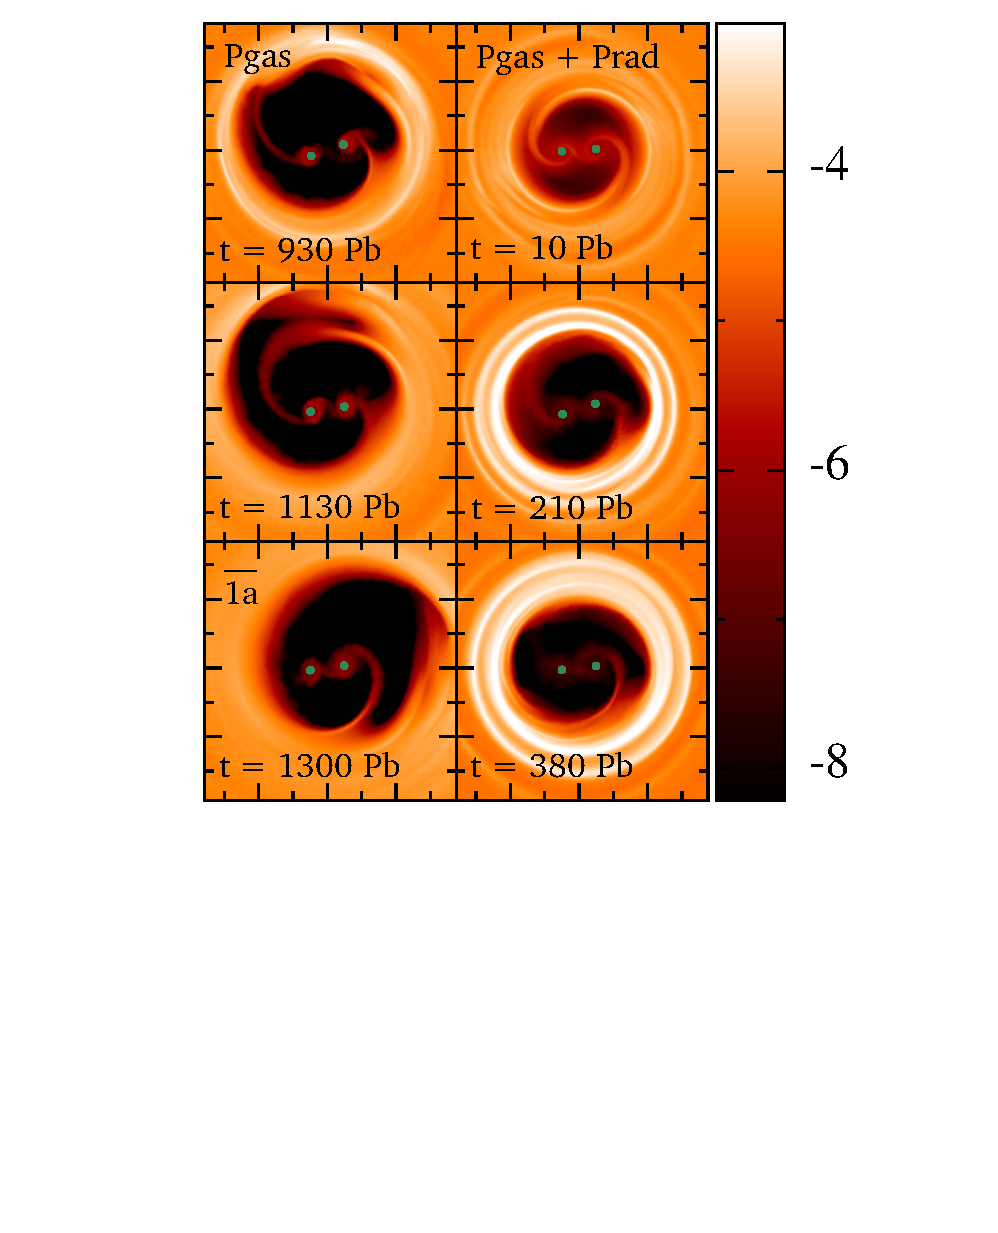
\includegraphics[width=\columnwidth, trim=3cm 6cm 2.2cm 0cm, clip]{Fig/disc/file-mod.pdf} \\
    \caption{Surface density map in IU in the $x-y$ plane for the simulation with $P_{\rm tot}=P_{\rm gas}$ (left column) and $P_{\rm tot}=P_{\rm gas}+P_{\rm rad}$ (right column). From the top to the bottom row: circular equal mass binaries at the beginning of the accretion process, after $200 \, P_{\rm B }$ and after more $180 \, P_{\rm B }$. In both the simulations, at $t=0$ the cavity radius is $2a_{\rm 0}$.
    In the absence of radiation pressure, the disc experiences a transient phase lasting around $900 \, P_{\rm B}$, during which the aspect ratio increases. This leads the binary to accreate gas from the cavity wall through the streams. However, when radiation pressure is considered, the binary system begins accreting material from the early stages of the evolution, forming mini discs after just 10 orbits. In this case, the mini discs covers a larger area compared to a scenario without radiation pressure. 
    After 200 orbits, in the simulation with radiation pressure, the mini discs appear weaker, in contrast to the simulation without radiation pressure, where the mini-discs remain full with a well distinguished shape. This distinction is also notable after an additional 180 orbits. 
    }
    \label{fig:disc}
    \end{center}
\end{figure}



\begin{figure}[h]
    \begin{center}
    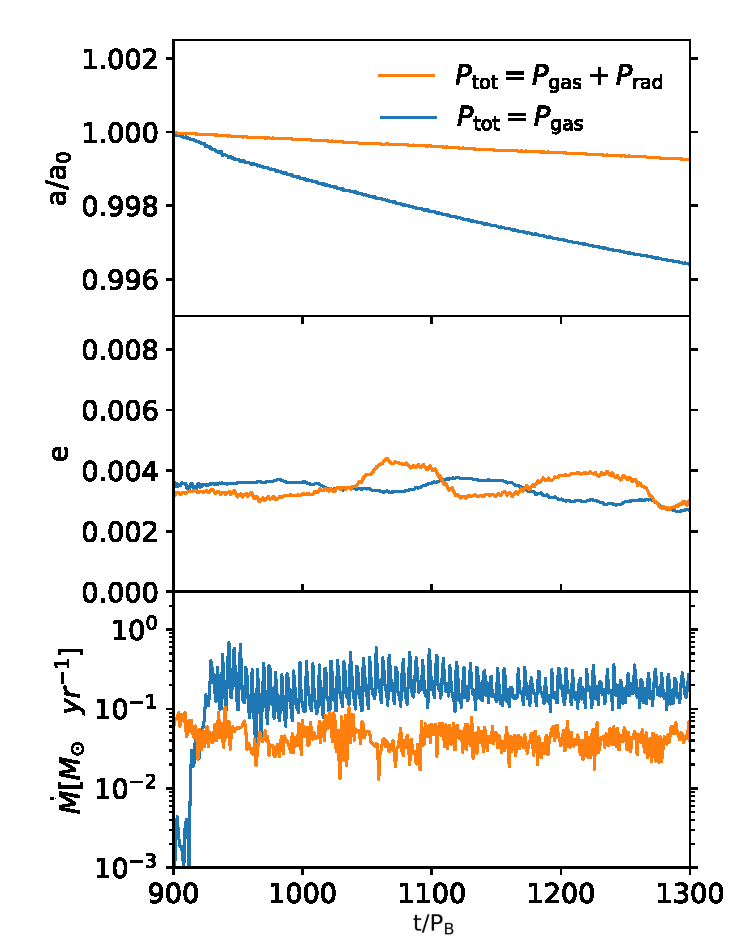
\includegraphics[width=\columnwidth]{Fig/Results/e0q1_hr01_md001aemdot.pdf} \\
    \caption{Time evolution of the semi-major axis (top panel), eccentricity (centre panel) and accretion rate (bottom panel) over the last 400 orbital periods. The orange and the blue lines refer to the simulation with and without the radiation pressure contribution, respectively. The semi-major axis is normalised to set $a(t=900  \, P_{\rm B}$)/$a_{0}$=1.
    In both cases the binary shrinks. In particular, when the ration pressure is implemented, the decreasing rate of the semi-major axis is lower. The eccentricity increases, reaching values approximately around 0.003. 
    When the radiation pressure is included in the simulation, after a transient phase of about 400 orbital periods, the $\dot M$ fluctuates around $0.03-0.04 \, \rm M_{\odot} \, yr^{-1}$. Instead, without the implementation of the radiation pressure, $\dot M$ is hogher with fluctuations around $0.1 \, \rm M_{\odot} \, yr^{-1}$.}
    \label{fig:a_e_mdot}
    \end{center}
\end{figure}


\begin{figure*}[h]
    \begin{center}
    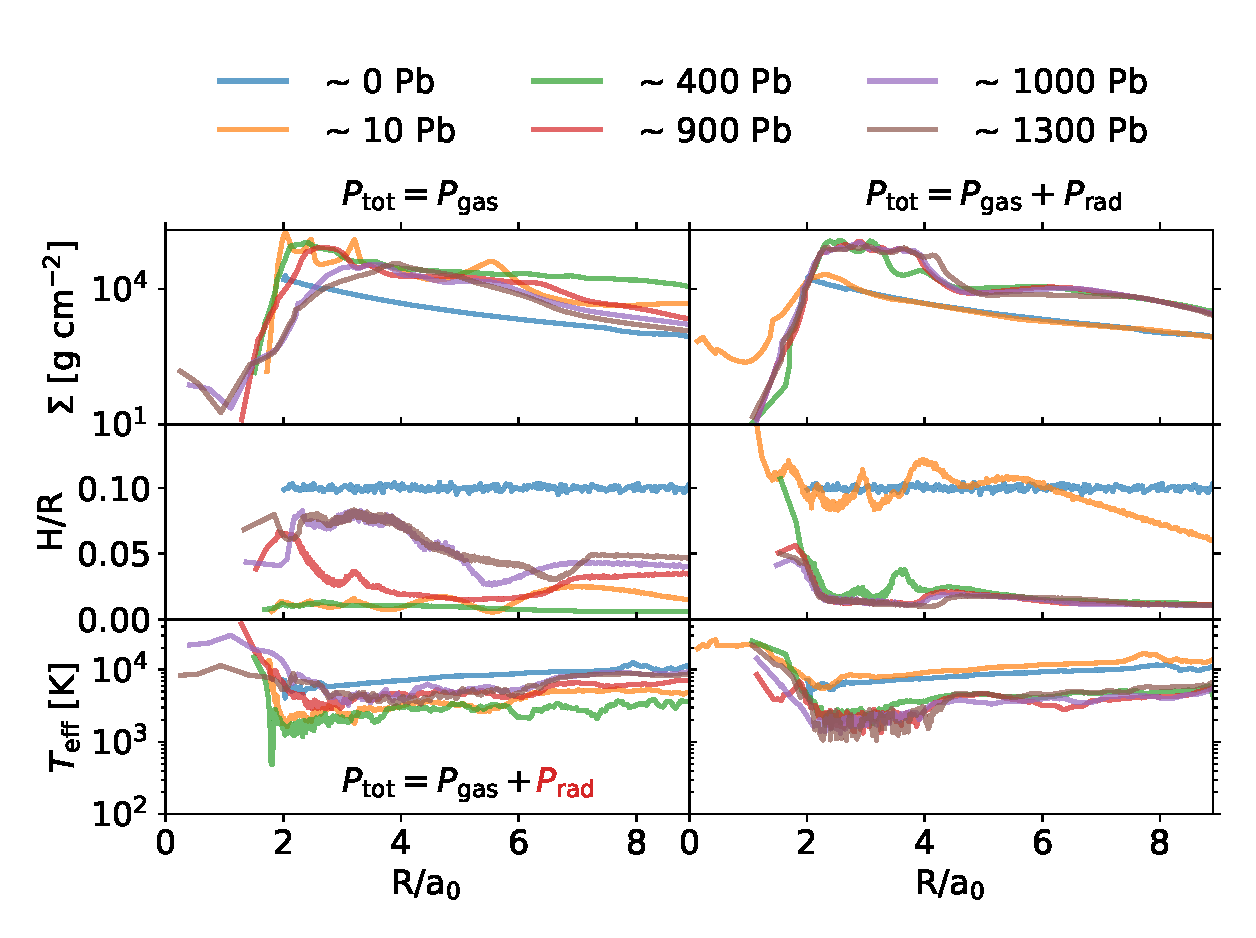
\includegraphics[width=1.8\columnwidth ]{Fig/Results/e0q1_hr01_md001all_Sigma_hr_Teff_prad.pdf} \\
    \caption{Time evolution of the surface density (first row), disc aspect ratio H/R (second row) and the effective temperature (third row) as a function of radius for the simulation without (left column) and with (right column) the implementation of the radiation contribution in the simulation code. We present the surface density, the thickness and temperature profiles at different times, distinguished by different colours. 
    surface density increases over the first 900 orbits and than decreases over the last 300 orbits, in particular in its inner part. In the mean time, the aspect ratio decreases during the transient phase and increase again eventually stabilising at constant values: in the inner part of the disc $H/R \sim 0.08$ while in the outer regions of the disc $H/R \sim 0.05$. We calculate the effective temperature assuming that both the gas and the radiation pressure contribute to the hydrostatic equilibrium of the disc. $T_{\rm eff}$  result to have an effective temperature between $[1,8]\times 10^{3} \, \rm K$.
    When $P_{\rm tot}=P_{\rm gas}+P_{\rm rad}$, the aspect ratio decreases over the first 400-500 orbital periods, reaching $H/R \sim 0.2-0.3$. The surface density increases in all the region of the disc and the effective temperature reaching values around $\sim 1-4 \times 10^3 \, K$. \fc{devo riscriverla mettendo come soggetto il disco e non le quantità}}
    \label{fig:hr_teff}  
    \end{center}
\end{figure*}

\begin{figure}[h]
    \begin{center}
    \label{} 
    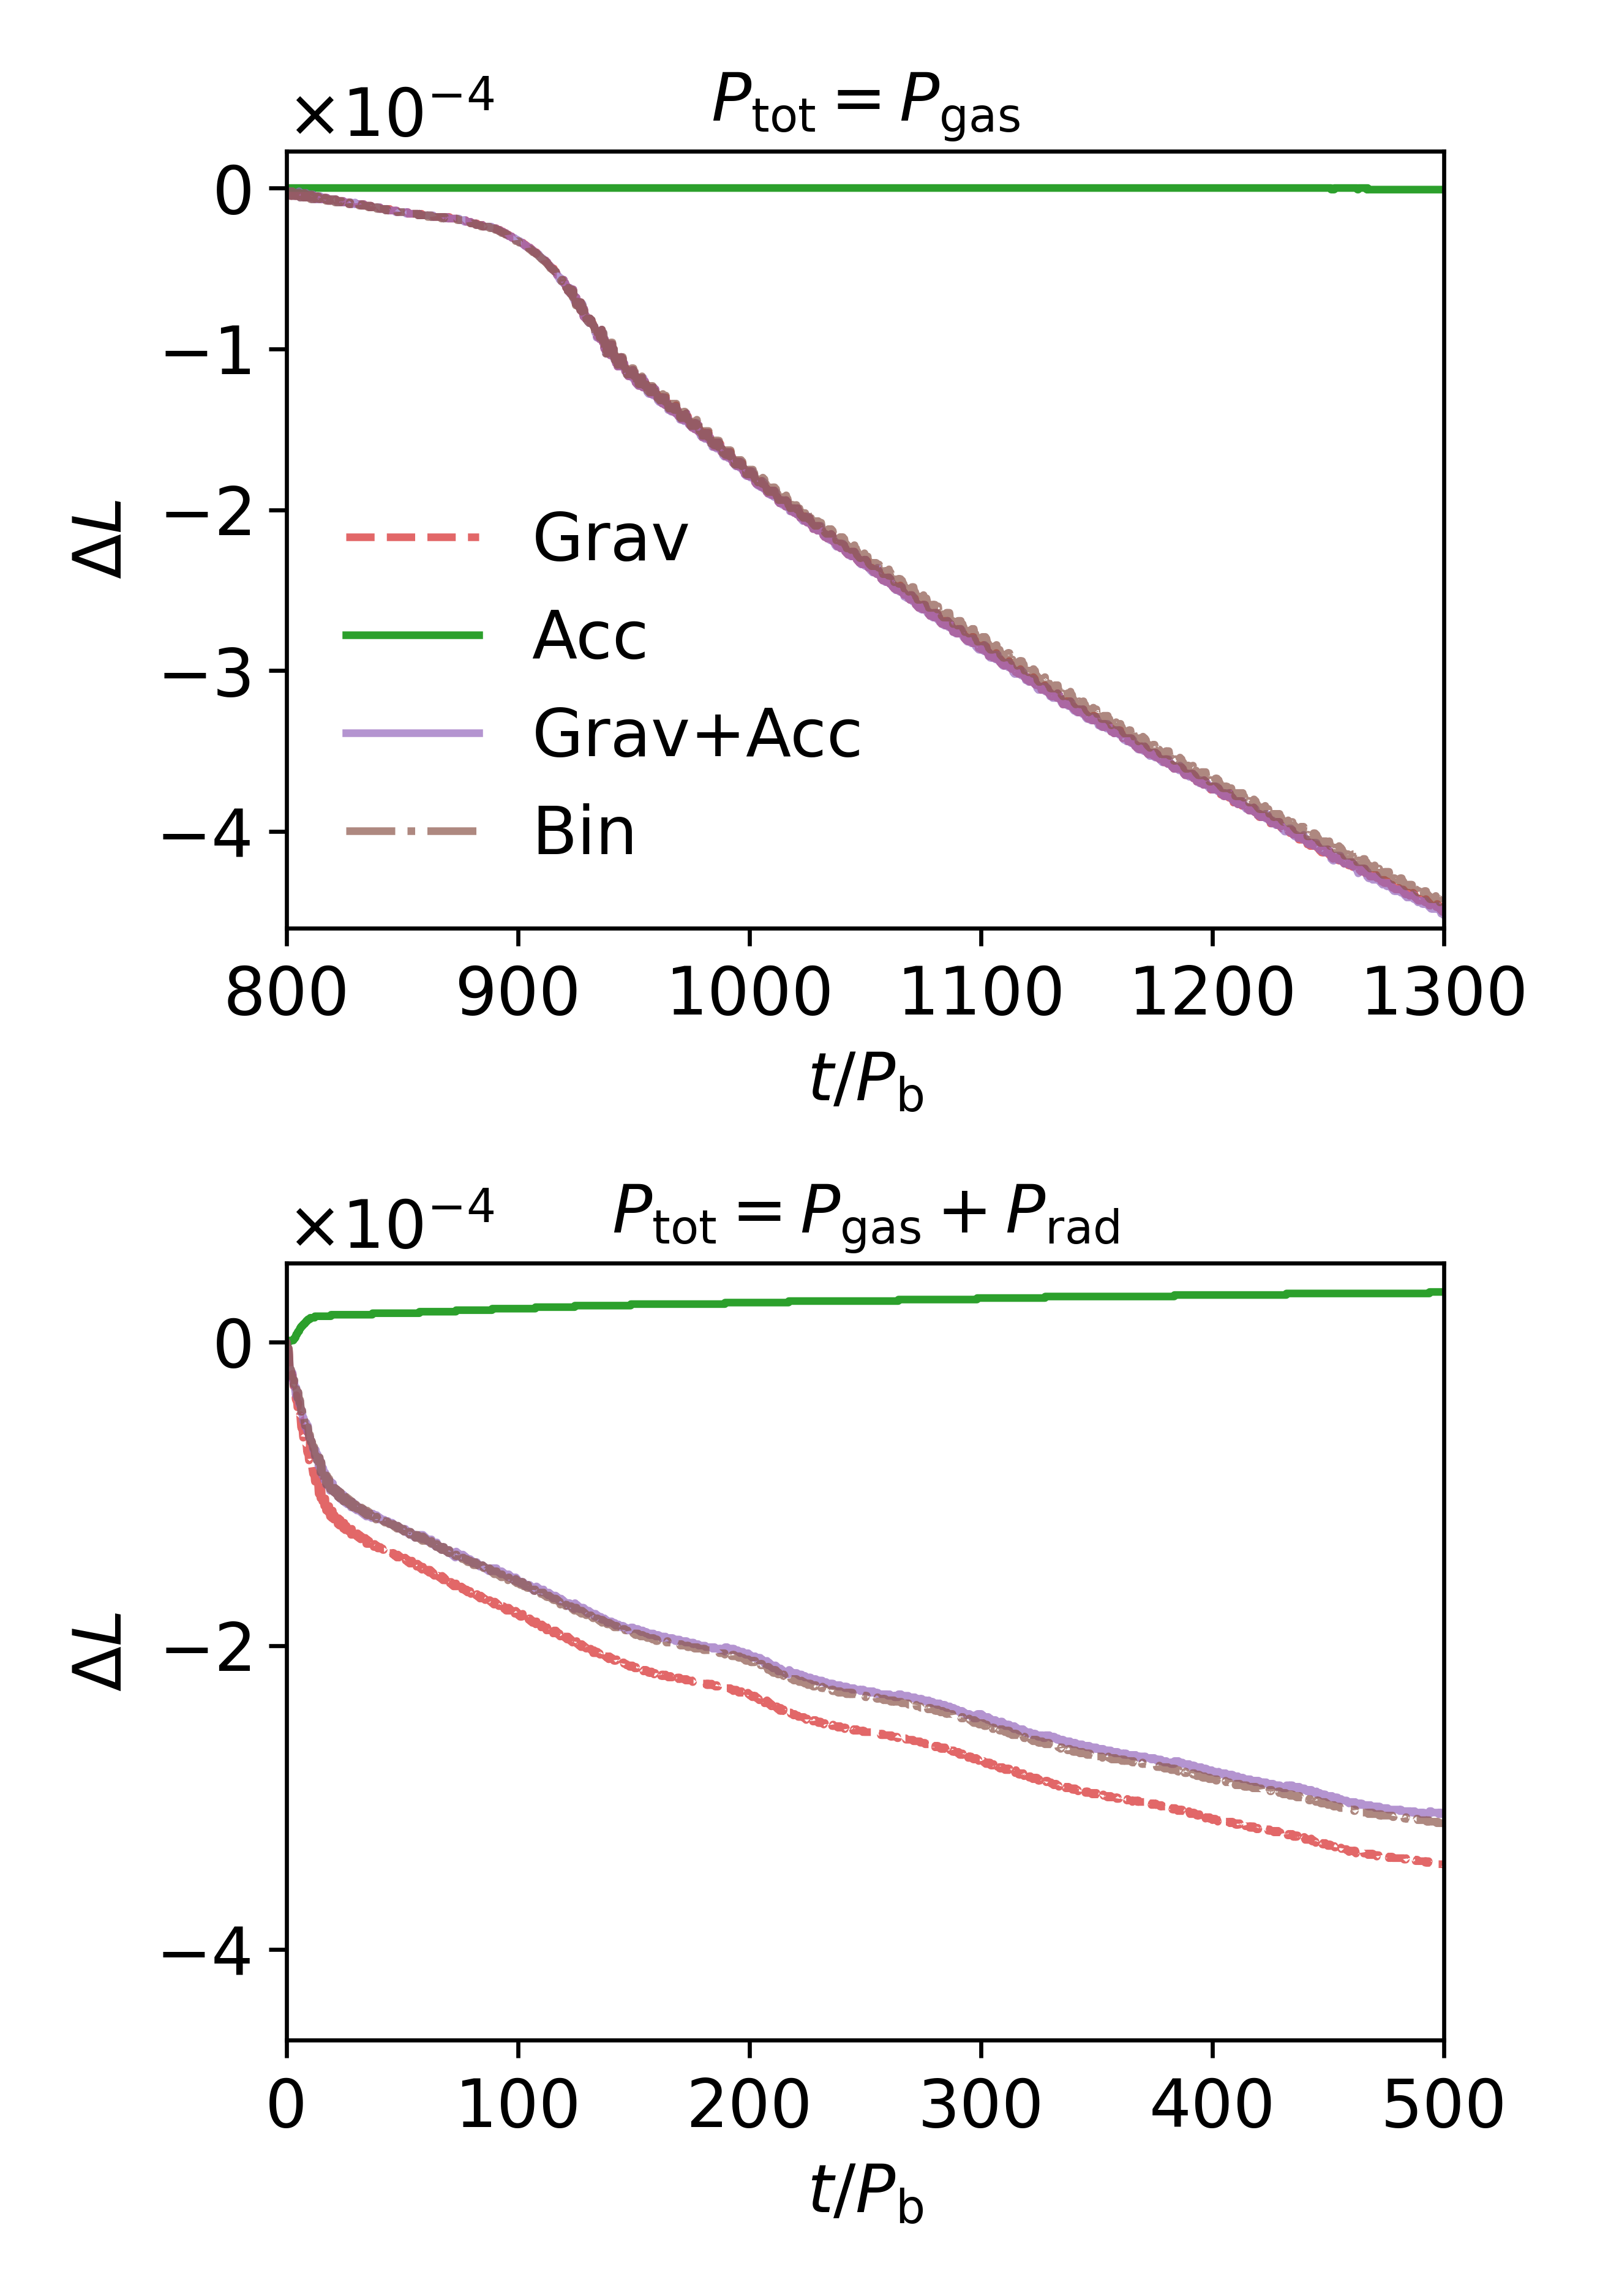
\includegraphics[width=\columnwidth]{Fig/Results/AngMom_Pgas_zoom.png} \\   
    \caption{}
    \end{center}
\end{figure}

\begin{figure}[h]
    \begin{center}
    \label{fig:ecc} 
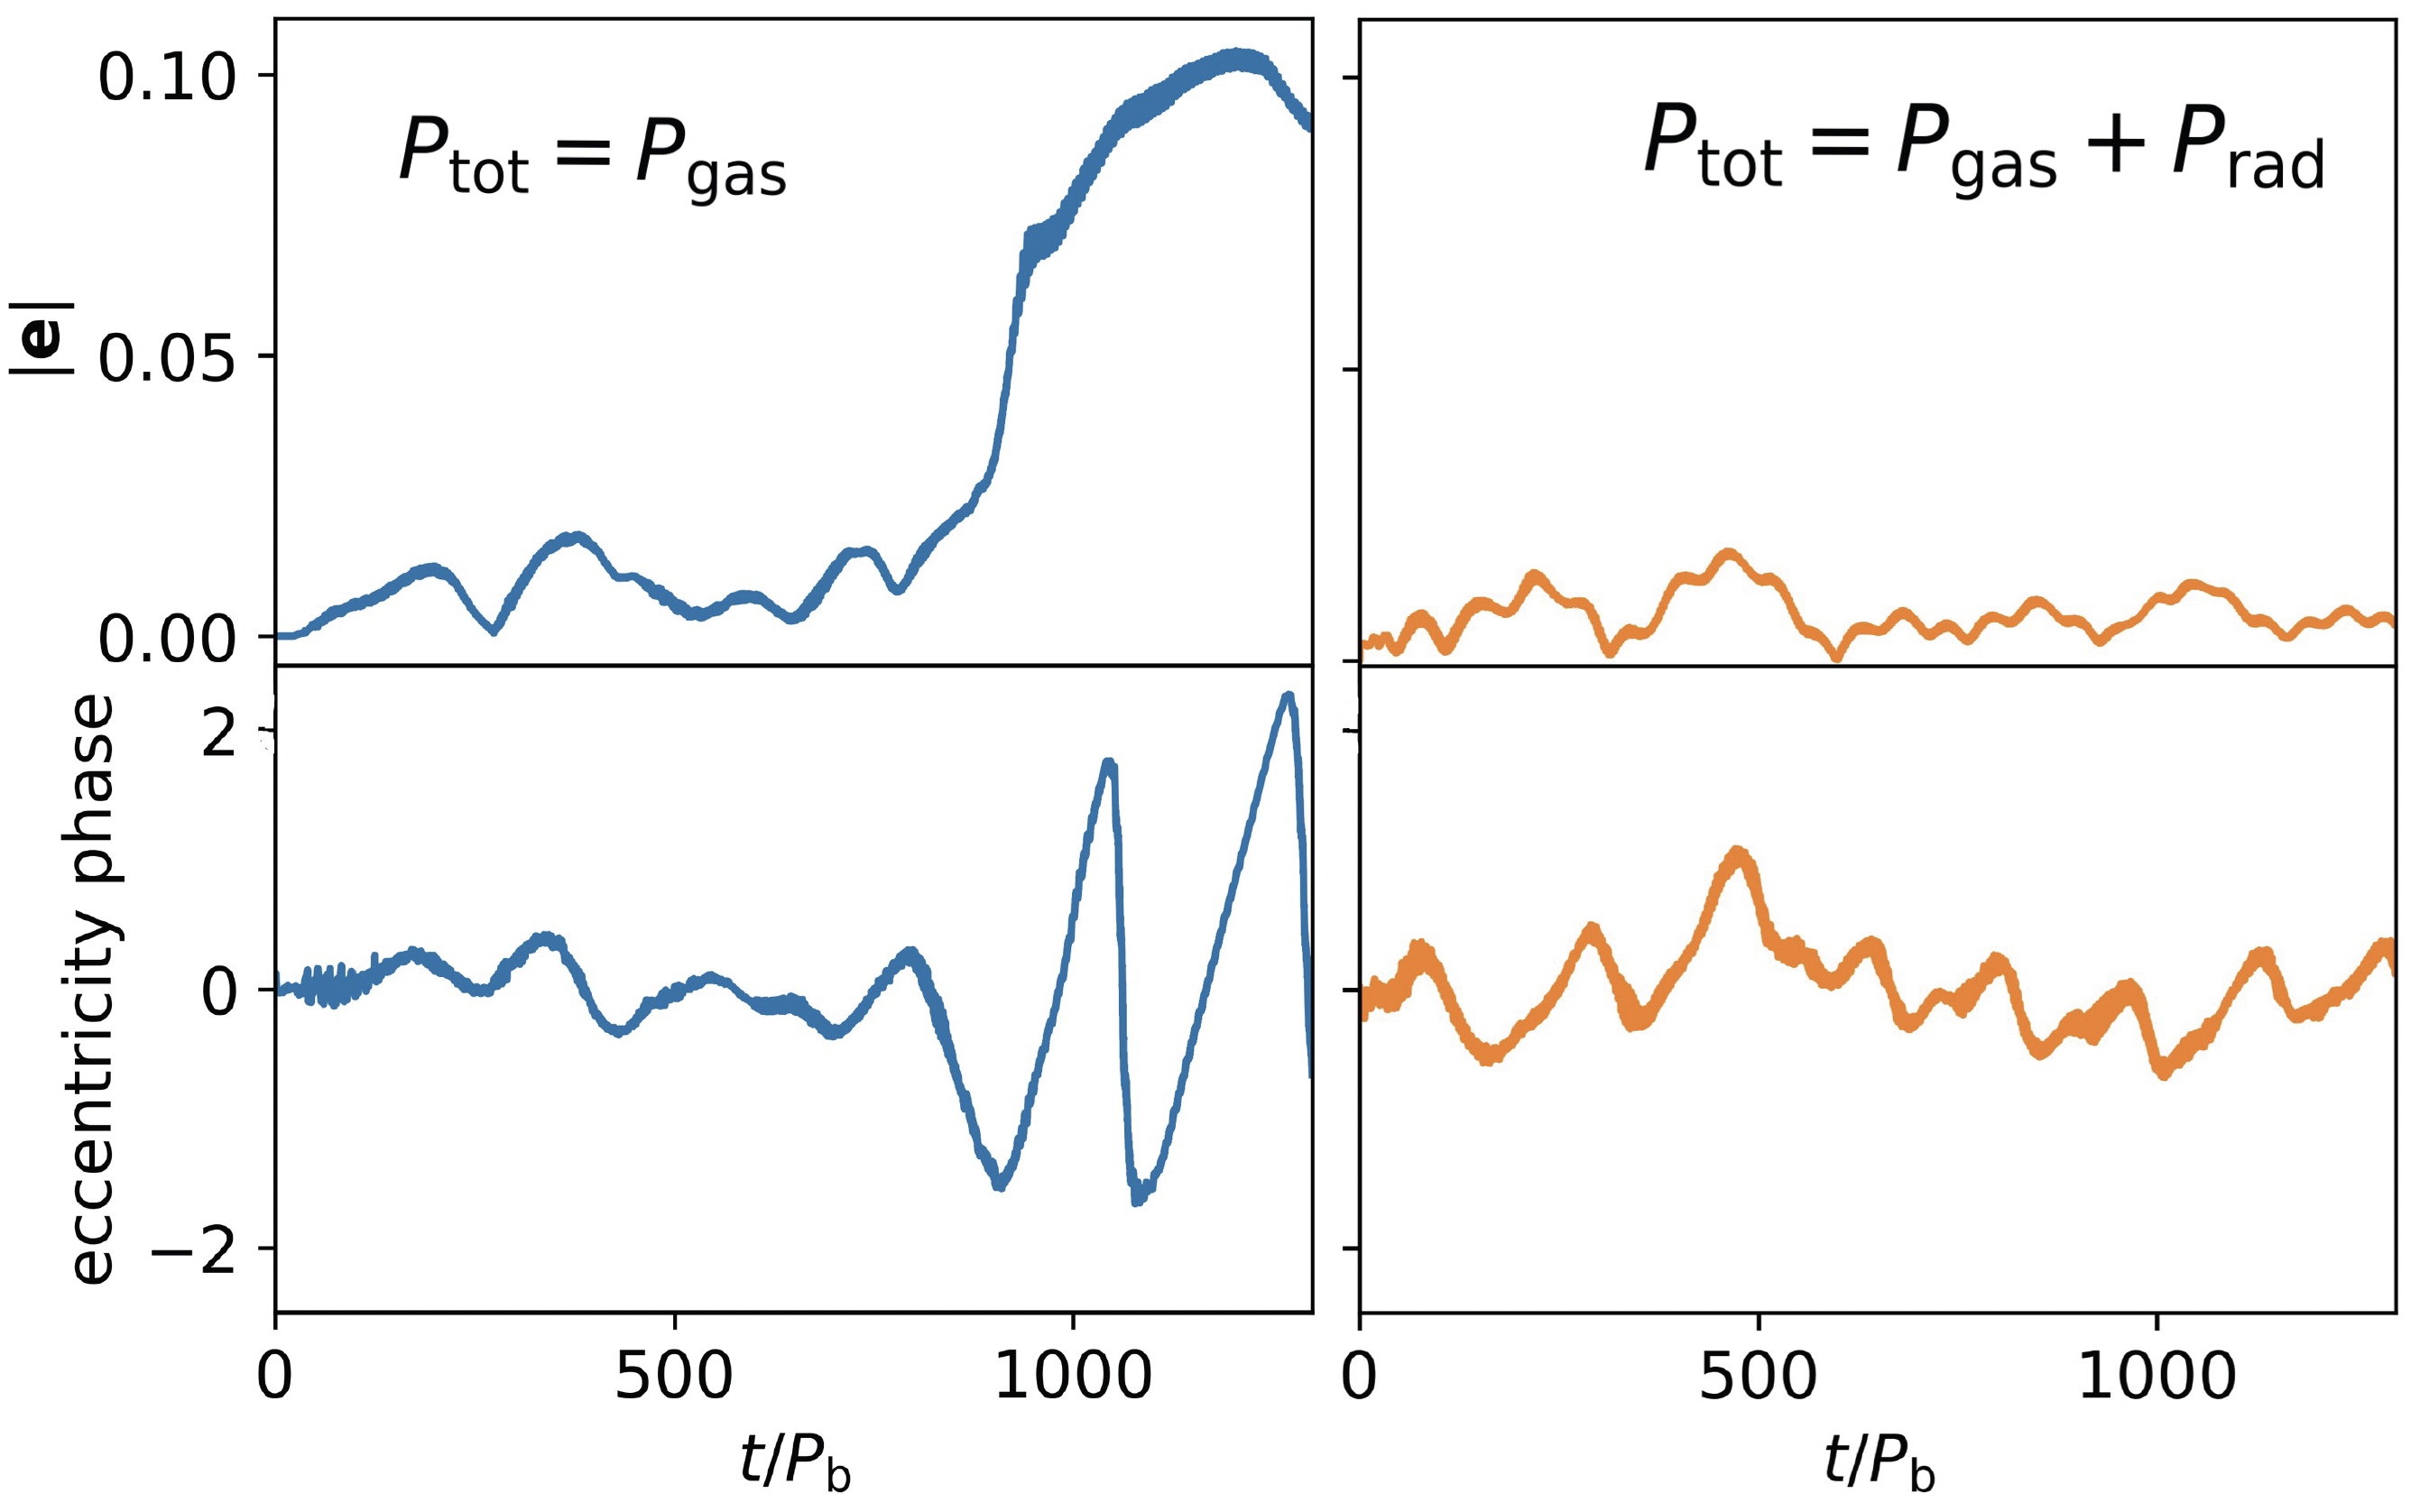
\includegraphics[width=\columnwidth]{Fig/Results/ecc.png} \\   
    \caption{Eccentricity vector evolution over time for the simulation without (left column) and with (right column) the implementation of the radiation contribution in the simulation code. The top panel shows the magnitude and the bottom panel shows the phase in radians. When the radiation pressure contributes to the hydrostatic equilibrium of the disc, the cavity remains circular and the precession is not significant as emerge when the radiation pressure is neglected.}
    \end{center}
\end{figure}

%%%%%%%%%%%%%%%%%%%%%%%%%%%%%%%%%%%%%%%%
%%%%%%%%%%%%%%%%% SEDs AND LCs %%%%%%%%%%%%%%%%%%
\subsection{Electromagnetic signatures}
\label{Results_SEDsLCs}

\begin{figure}[h]
    \begin{center}
    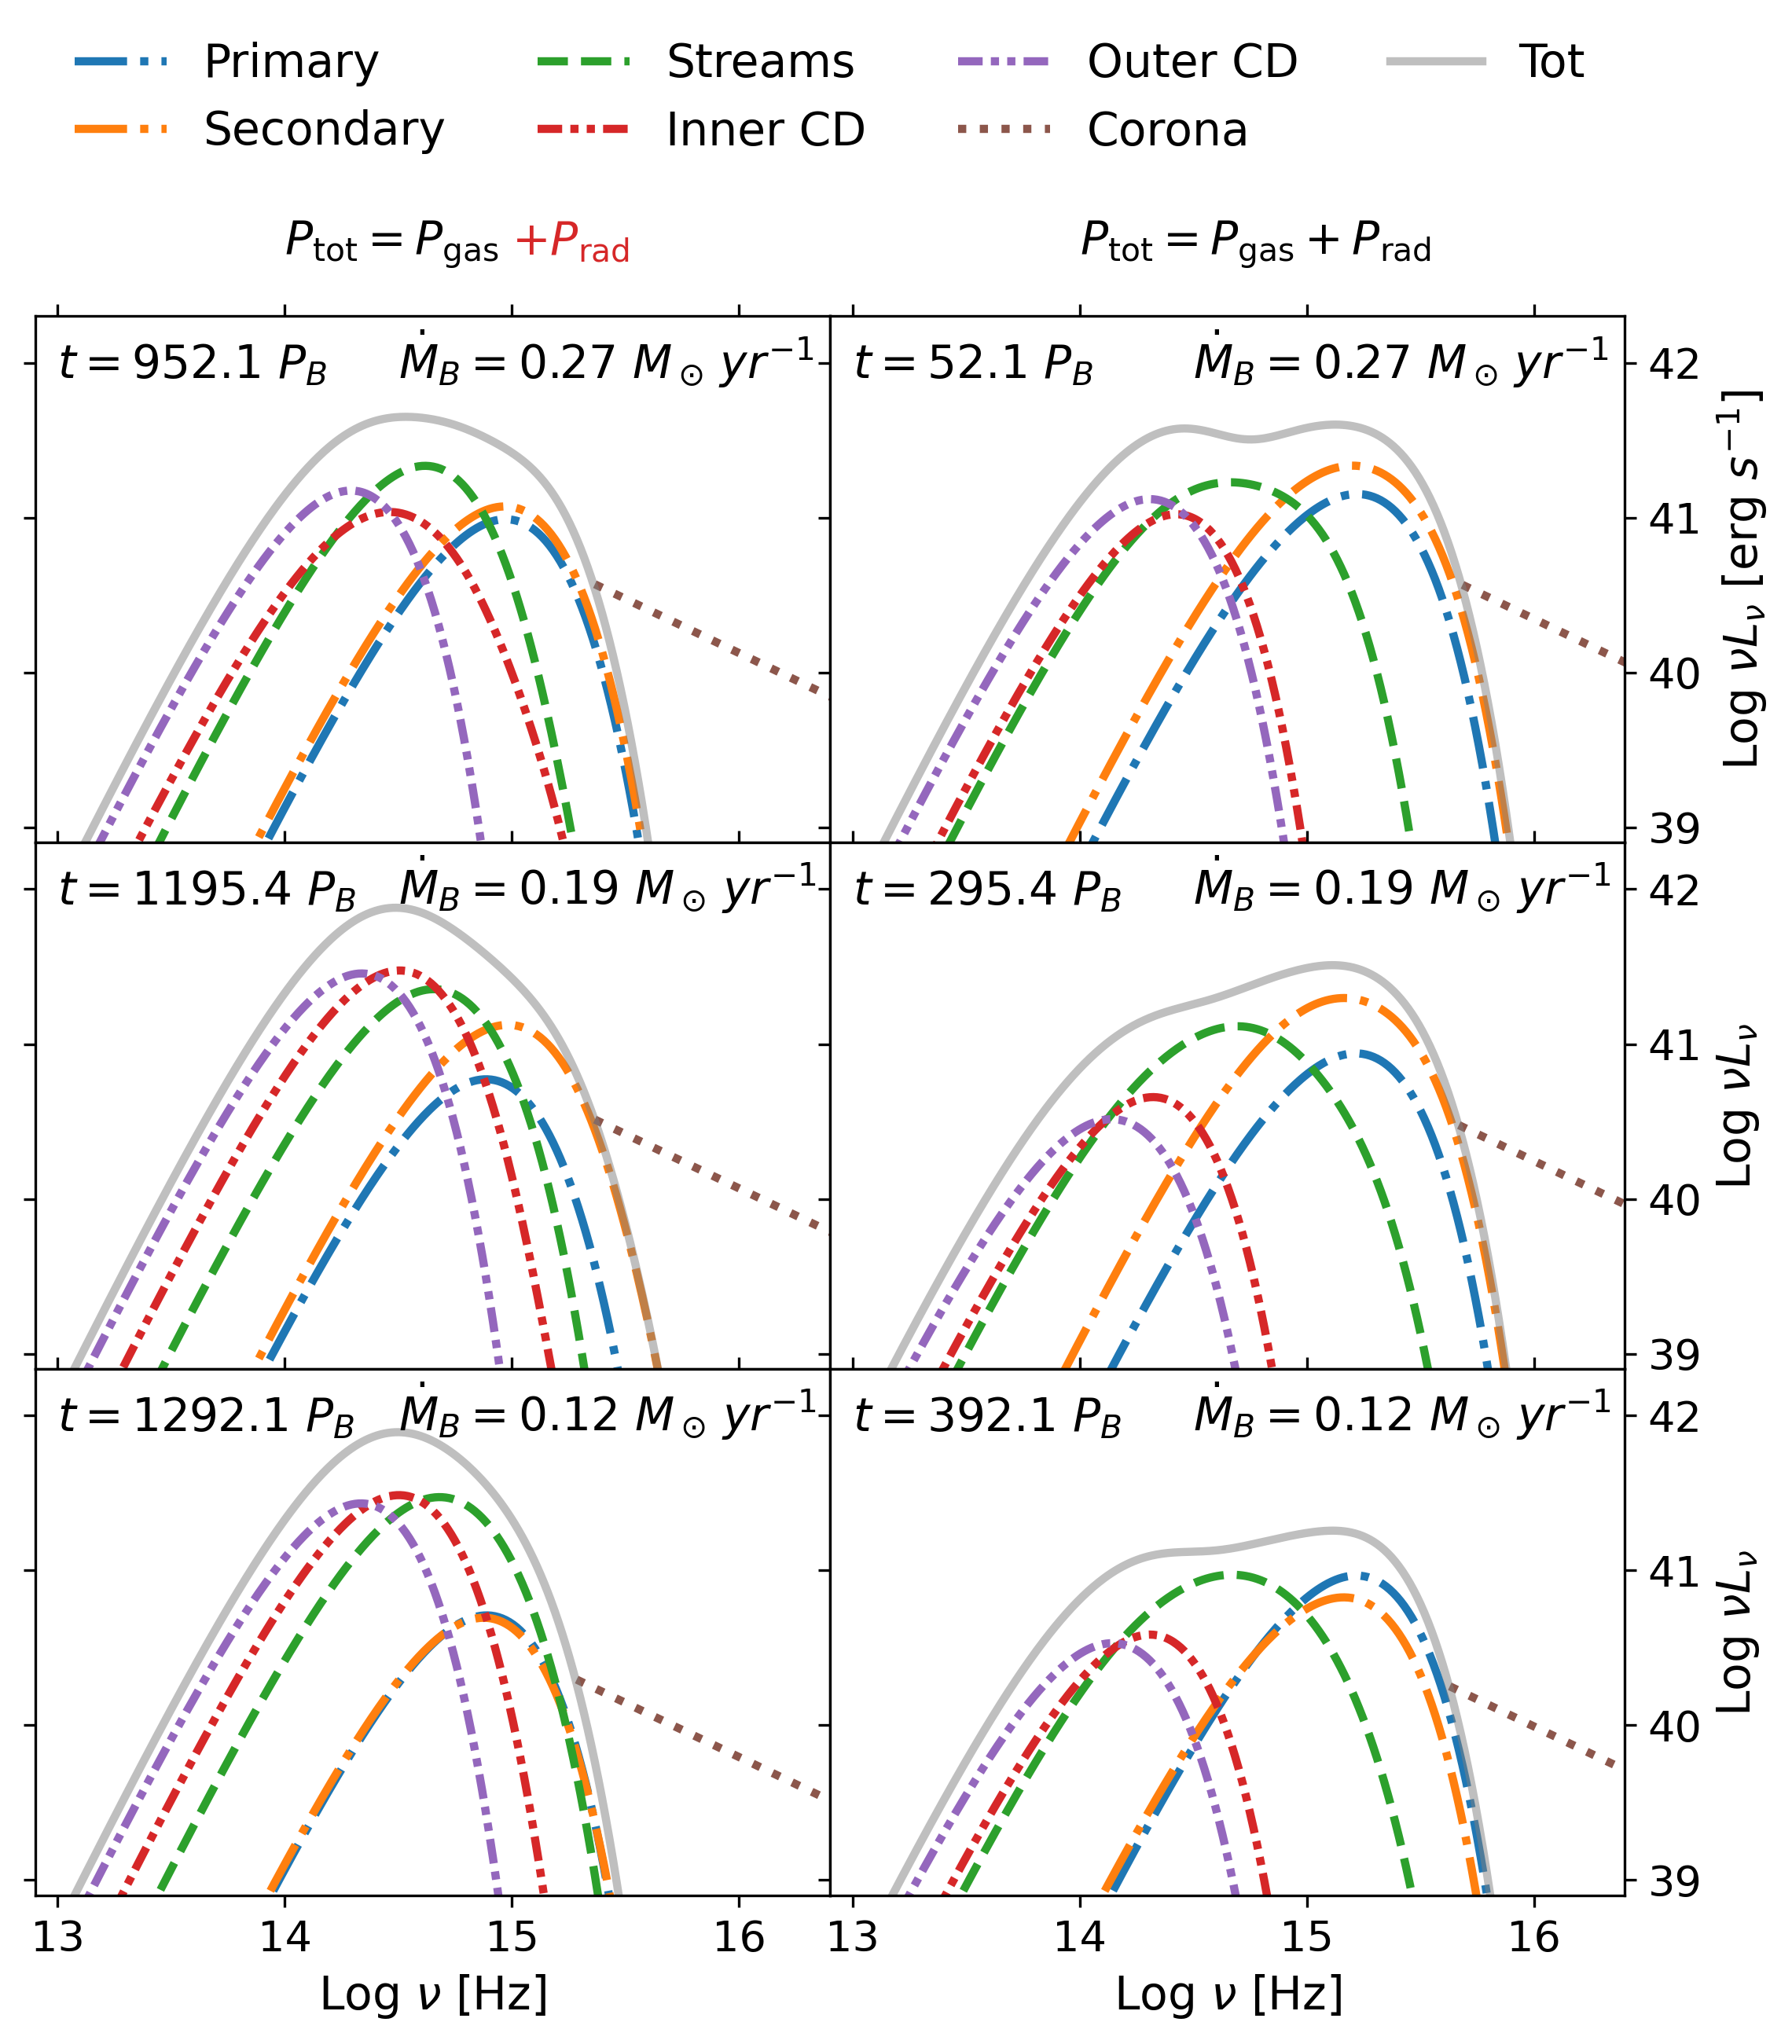
\includegraphics[width=\columnwidth]{Fig/Results/q1e0_prad_hr01_md001_rOut10_3921_PgasPrad_comparison.png} \\
    \caption{Comparison between the spectral energy distributions (SEDs) obtained by including the contribution of the radiation pressure either a posteriori (left column) or during the binary evolution (right panel) at the same accretion rate. The first row shows the the contribution from the different regions of the disc (e.g. mini-discs, stream, inner and outer part of the circumbinary disc and the corona) in different colours when the accretion rate of both binaries is $\dot M _{\rm B} = 0.27 \, \rm M_{\odot} \, yr^{-1}$. The second and third rows display the SEDs computed at $\dot M _{\rm B} = 0.19 \, \rm M_{\odot} \, yr^{-1}$ and $0.12 , \rm M_{\odot} \, yr^{-1}$, respectively.
\fc{aggiungere commento sulla luminosità, differenza di contrubiti del disco e mini disc, spettri dei md con range di nu più ampio nei casi con prad}.}
    \label{fig:SED}
    \end{center}
\end{figure}

\begin{figure}[h]
    \begin{center}
    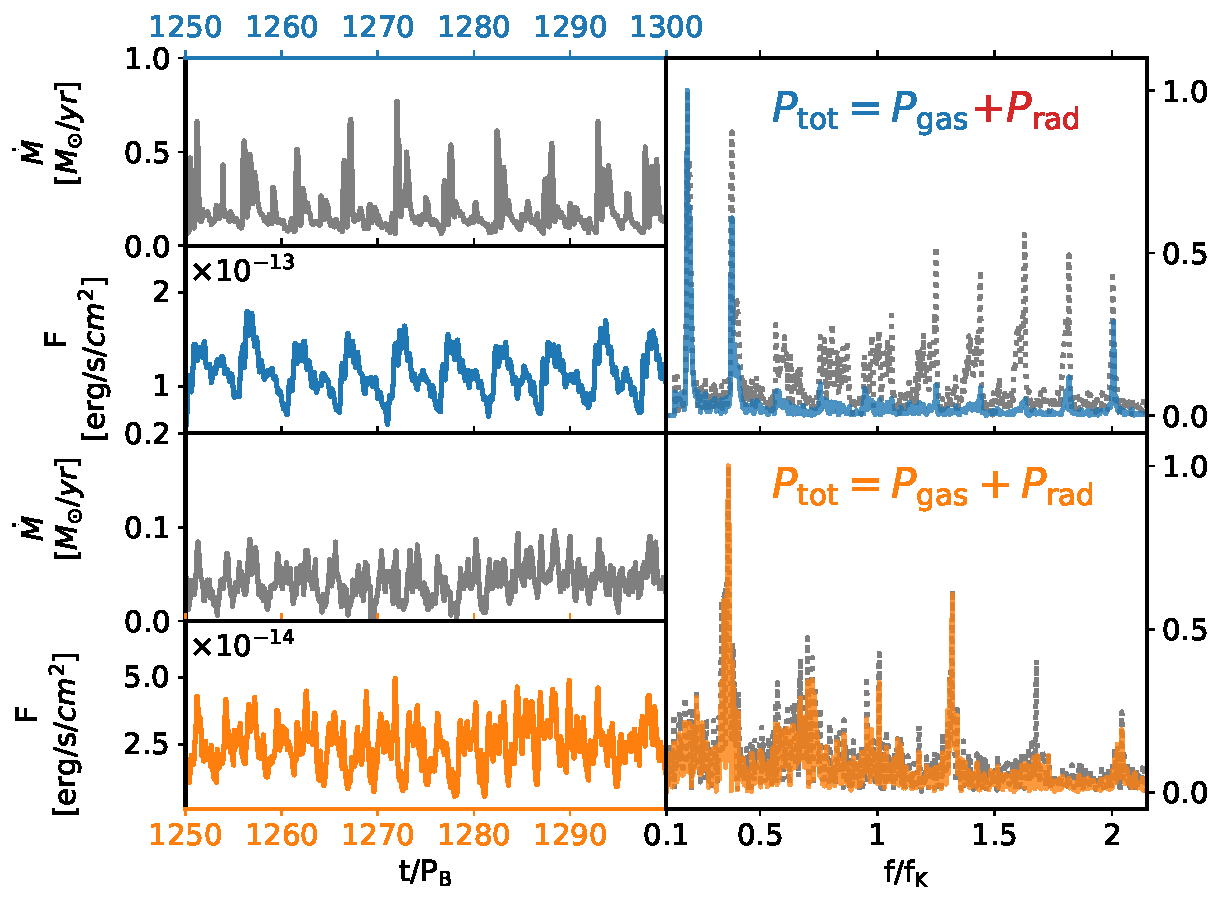
\includegraphics[width=\columnwidth ]{Fig/Results/e0q1_hr01_md001OpticAll_Flux_bands_10000_0.1_comparisonPgasPras.pdf} \\
    \caption{Light curves for circular equal mass binaries at z=0.1. The top left panels show the evolution of accretion rate (grey line) and the flux (blue line) in the optical G band, over 50 orbits within the time window $t=1250-1300 \, P_{\rm B}$ for the case where the radiation pressure is included a posteriori. On the top right, are shown the FFT of these quantities over 100 orbits, in the time domain $t=1200-1300 \, P_{\rm B}$, normalised to unity, in function of $f/f_{\rm K}$ where $f_{\rm K}$ the Keplerian frequency of the binary. The bottom panels show the accretion rate, the flux in the optical G band the FFT of these quantities in the case where the radiation pressure is implemented in the simulation of the binary evolution. In this scenario, the accretion rate and the flux are illustrated in the time domain $t=1250-1300 \, P_{\rm B}$ and the FFT is computed over the time domain $t=1200-1300 \, P_{\rm B}$. In both the cases, the optical G flux is computed taking into account an extra Gaussian noise. \fc{aggiungere commenti su differenze}}
    \label{fig:LCs_FFT}  
    \end{center}
\end{figure}

%%%%%%%%%%%%%%%%% CONCLUSION %%%%%%%%%%%%%%%%%%

\section{Conclusions}
\label{sec:conclusions}


%%%%%%%%%%%%%%%%% ACNOWLEDGEMENTS %%%%%%%%%%%%%%%%%%
\section*{Acknowledgements}

We thank Daniel Price for providing the {\sc phantom} code for numerical simulations and acknowledge the use of {\sc splash} \citep{Price2007} for the rendering of the figures.
We thank Phil Hopkins for providing the {\sc gizmo} code for numerical simulations. 
AF and AS acknowledge financial support provided under the European Union’s H2020 ERC Consolidator Grant ``Binary Massive Black Hole Astrophysics" (B Massive, Grant Agreement: 818691). AL acknowledges support by the PRIN MUR "2022935STW".


%%%%%%%%%%%%%%%%%%%%%%%%%%%%%%%%%%%%%%%%%%%%%%%%%%

% WARNING
%-------------------------------------------------------------------
% Please note that we have included the references to the file aa.dem in
% order to compile it, but we ask you to:
%
% - use BibTeX with the regular commands:
%   \bibliographystyle{aa} % style aa.bst
%   \bibliography{Yourfile} % your references Yourfile.bib
%
% - join the .bib files when you upload your source files
%-------------------------------------------------------------------
\bibliographystyle{aa} % style aa.bst
\bibliography{bibliography}
\end{document}
%
%%%%%%%%%%%%%%%%%%%%%%%%%%%%%%%%%%%%%%%%%%%%%%%%%%%%%%%%%%%%%%
Example below of non-structurated natbib references  
To use the v8.3 macros with this form of composition of bibliography, 
the option "bibyear" should be added to the command line 
"\documentclass[bibyear]{aa}".
%%%%%%%%%%%%%%%%%%%%%%%%%%%%%%%%%%%%%%%%%%%%%%%%%%%%%%%%%%%%%%
%%%%%%%%%%%%%%%%%%%%%%%%%%%%%%%%%%%%%%%%%%%%%%%%%%%%%%%%%%%%%%
Examples for figures using graphicx
A guide "Using Imported Graphics in LaTeX2e"  (Keith Reckdahl)
is available on a lot of LaTeX public servers or ctan mirrors.
The file is : epslatex.pdf 
%%%%%%%%%%%%%%%%%%%%%%%%%%%%%%%%%%%%%%%%%%%%%%%%%%%%%%%%%%%%%%


\begin{appendix} %First appendix
%
\longtab[1]{
\begin{landscape}
\begin{longtable}{lrcrrrrrrrrl}
...
\end{longtable}
\end{landscape}
}% End longtab
\end{appendix}

%%%% End of aa.dem
